\begin{figure}[!ht]
\centering
% https://docs.google.com/presentation/d/109vfeK_lHSsE0q7Iz7tzl9sDxnP8jyOF2gJ-v85pgL8/edit?usp=sharing
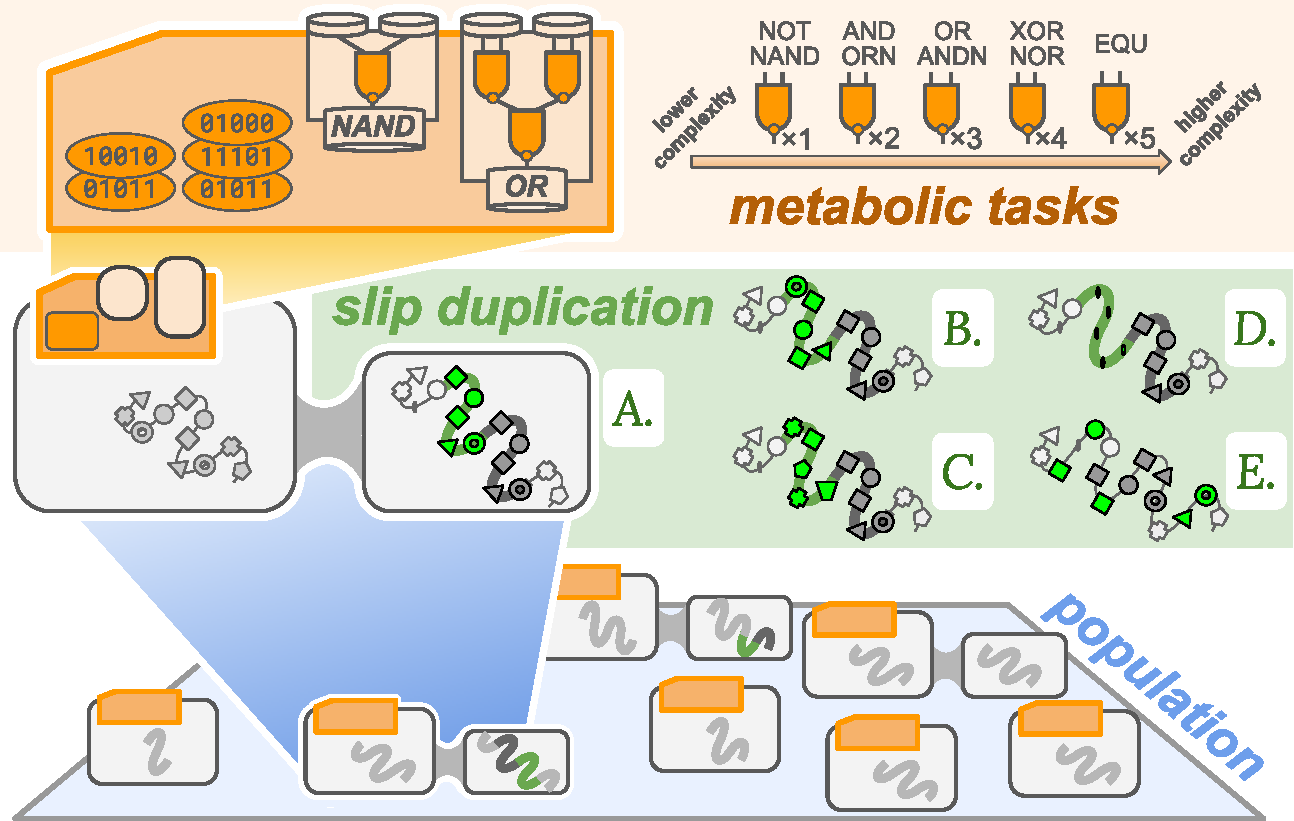
\includegraphics[width=\linewidth]{imgs/GeneDupeOps.pdf}
\caption{%
\textbf{Genome replication and phenotypic traits in Avida.}
\footnotesize
Self-replicating computer programs serve as digital model organisms.
Organisms comprise virtual stacks and registers used to store binary values and pointers within a circular genome of program instructions used to track instruction execution and copying.
Competition to survive and reproduce occurs within a limited-capacity population.
Replication activity can be accelerated by carrying out available ``metabolic' input/output tasks.
% @AML: Readers might not know what is meant by "gates"; would lean toward "instructions" instead.
These tasks vary in complexity with respect to the number of NAND operations required to perform them.
An organism's metabolic ``phenotype'' arises from the expression of its genetic code.
Genetic code copied from parent to offspring may be subject to point mutations, which change the individual instruction values, and slip mutations, which introduce or remove many instructions all at once.
Reported experiments compare five alternate variants of slip mutation:
A) \textit{Slip-duplicate}, an exact duplication is inserted adjacent to the target segment;
B) \textit{Slip-scramble}, shuffled duplication is inserted directly after the target segment;
C) \textit{Slip-random}, random instructions are inserted directly after the target segment;
D) \textit{Slip-NOP}, neutral nop-X instructions are inserted directly after the target segment; and
E) \textit{Slip-scatter}, randomly-drawn instructions are inserted at random throughout the genome.
}
\label{fig:slip_mut_variants}
\end{figure}
